\documentclass{article}

\usepackage{amsmath,amssymb}
\usepackage{hyperref}
\usepackage{amssymb}
\usepackage{graphicx}
\graphicspath{{../logos/}}


\begin{document}

\setlength{\tabcolsep}{0.015\textwidth}
\begin{center} \begin{tabular}{cccc}
	
\includegraphics[width=0.16\textwidth]{SAMF_logo.jpg} &
	
\includegraphics[width=0.35\textwidth]{SAICA_logo.jpg} &
	
\includegraphics[width=0.18\textwidth]{Liberty_logo.jpg} &
	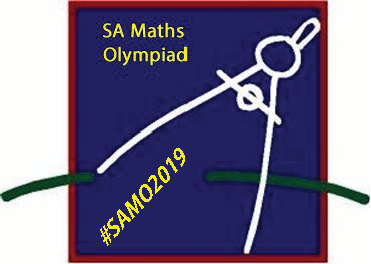
\includegraphics[width=0.18\textwidth]{SAMO2019.png}
\end{tabular} \end{center}

\bigskip

\begin{center}
\textbf{\Large Senior January Monthly Problem Set}
\\ \vspace{1em}
\textbf{\large Due: Friday, 17 January 2020}
\end{center}


\begin{enumerate}

\bigskip
\item[1.] %PAMO Shortlist 2019
On the board, we write the integers $1, 2, 3, \dots, 2019$.
At each minute, we pick two numbers on the board $a$ and $b$, erase them, and write down the number $s(a + b)$ instead where $s(n)$ denotes the sum of the digits of the integer $n$.
Let $N$ be the last number remaining on the board.
\begin{enumerate}
	\item Is it possible that $N = 19$?
	\item Is it possible that $N = 15$?
\end{enumerate}


\medskip
\item[2.] %Baltic Way 2009 Problem 8
For which positive integers $n$ is it possible to divide the set of numbers $\{n, n+1, n+2, \dotsc, n+8\}$ into two disjoint sets $A$ and $B$ such that the product of the numbers in $A$ is equal to the product of the numbers in $B$?


\medskip
\item[3.] % Liam
Let $M$ be a positive integer, and let $S$ denote the set of finite sequences of positive integers less than or equal to $M$, including the empty sequence of length zero, which we denote as $\mathbf{0}$.
Also, for a sequence $\mathbf{x} = (x_1, x_2, \dotsc, x_n)$ let $\overline{\mathbf{x}}$ denote the reverse sequence $\overline{\mathbf{x}} = (x_n, x_{n-1}, \dotsc, x_1)$.

Define a function $d$ from $S$ to the integers as follows:
\begin{itemize}
\item $d(\mathbf{0}) = 0$.
\item If $\mathbf{x} = (x_1, x_2, \dotsc, x_n)$ is a sequence of positive length, let $m$ be the largest integer such that $x_1 +x_2 +\dotsb +x_m \leq M$, and let $\mathbf{x}'$ denote the rest of the sequence: $\mathbf{x}' = (x_{m+1}, \dotsc, x_n)$.
Then $d(\mathbf{x}) = 1 +d(\mathbf{x}')$.
\end{itemize}
Show that $d(\mathbf{x}) = d(\overline{\mathbf{x}})$.


\medskip
\item[4.]
Let $ABCD$ be a cyclic quadrilateral with its diagonals intersecting at $E$.
Let $M$ be the midpoint of $AB$.
Suppose that $ME$ is perpendicular to $CD$.
Show that either $AC$ is perpendicular to $BD$ or $AB$ is parallel to $CD$.


\medskip
\item[5.] % IMO 2008 Shortlist C3
We have done it! We have planted an infinite number of trees on the vertices of an infinite regular grid, one for each vertex. Let $T$ be a positive integer. 
We define a \textit{T-forest} as a set of trees such that for any two trees in the $T$-forest, there exists another tree planted in the grid such that the area of the triangle with these three trees as vertices is $T$.

What is the smallest $T$ such that our $T$-forest has more than $200$ trees?


\medskip
\item[6.] % IMO 2009 Shortlist N4
Given a series $t_1, t_2, \dotsc, t_n$ such that 
\[ t_{k + 1} = \frac{t_k^2 + 1}{t_{k-1} + 1} - 1 \quad \forall \ k \in \{2, 3, \dots, n - 1\}. \]
For which $n \in \mathbb{N}$ does there exist a $t_1$ and $t_2$ such that $t_i \in \mathbb{N}$ for all $i \in \{1, 2, 3, \dotsc, n\}$?


\medskip
\item[7.]
Let $AB$ and $CD$ be two chords of a circle $\Gamma$ that intersect at $X$ in the interior of $\Gamma$.
Let $\Gamma_1$ and $\Gamma_2$ be circles that are mutually tangent at $X$ and are tangent to $\Gamma$ at $P$ and $Q$.
Let $\omega$ be a circle tangent to $\omega_1$ and $\omega_2$ at $X$ that intersects the chords $AB$ and $CD$ at $M$ and $N$ respectively.
Prove that 
\[
	\frac{MP}{MQ} = \frac{NP}{NQ} \implies \angle AXM = \angle DMN.
\]

\medskip
\item[8.] % The Andrew and The Dylan
Let $n$ be a positive integer greater than $1$, and consider a circle of radius $1$ in which is inscribed a regular $n$-gon $P$ with vertices labelled from $1$ to $n$ in that order.
Consider the set $S$ of positive divisors of $n$, and the convex polygon $G$ formed by the points of $P$ with labels in $S$.
If the area of $G$ is denoted by $|G|$, show that
\[ 
	|G| < \frac{3}{2}.
\]

\end{enumerate}

\vfill
\textbf{\Large Email submission guidelines}
\begin{itemize}
	\item Email your solutions to \href{mailto:samf.training.assignments@gmail.com}{\texttt{samf.training.assignments@gmail.com}}.
	\item In the subject of your email, include your name and the level of the assignment (Beginner, Intermediate or Senior).
	\item Submit each question in a single separate PDF file (with multiple pages if necessary), with your name and the question number written on each page.
	\item If you take photographs of your work, use a document scanner such as Office Lens to convert to PDF.
	\item If you have multiple PDF files for a question, combine them using software such as PDFsam.
\end{itemize}

\end{document}
